\documentclass{homework}
\usepackage{marvosym}
\usepackage{hyperref}
\usepackage{color}
\usepackage{caption}
\usepackage{subcaption}
\usepackage{float}

\course{Algorithmische Bioinformatik}
\semester{Wintersemester 2012 / 2013}
\no{11}
\date{Montag, dem 14. Januar 2013}
\author{Stefan Meißner (4279113) und Niels Hoppe (4356370)}
\tutorial{Dienstag 08:00 - 10:00}
\tutor{Alena van Bömmel (Übungsgruppe 3)}

\begin{document}
\maketitle
\begin{enumerate} 

\aufgabe{Statistische Verteilungen}{30}
\begin{enumerate}
\item 
Vulkane brechen zufällig (je nach Vulkan in einem unterschiedlichen Zeitraum) aus. 
Um die Ausbrüche auf den Zeitraum von einem Jahr zu beziehen, bietet sich die Poisson-Verteilung an.
\item 
Bei Hochleistungssport ist davon auszugehen, dass alle Athleten ungefähr die gleiche Leistung bringen.
Die Sieger werden nur einige wenige Zentimeter weiter und die Letzten nur einige wenige Zentimeter weniger springen als der Rest.
Daher kann hier von einer Normalverteilung ausgegangen werden.
\item
Wir kennen uns leider mit dem Wachstum von Hefe nicht aus. Wenn diese ungefähr gleich schnell Wachsen, dann wird sich ein Mittelwert des Durschnitts ergeben. Hier wäre also eine Gauss-Verteilung angebracht.\\
Interessant ist aber auch:
Wikipedia: \textit{Da die Exponentialverteilung auch als Lebensdauerverteilung verwendet wird, ist es möglich,
damit zusammenhängende Größen wie Überlebenswahrscheinlichkeit,
die Restlebensdauer und die Ausfallrate mit Hilfe der Verteilungsfunktion anzugeben.}
Evtl. fallen auch einige Hefezellen komplett raus oder wachsen nicht mehr weiter bzw. andere deutlich schneller. Dann könnte man auch die Exponentialverteilung nutzen.
\end{enumerate}

\aufgabe{Gibbs Sampler}{30}

Beim Gibbs Sampling werden verschiedene Stichproben-Sequenzen einer DNA untersucht. U.a. soll herausgefunden werden, ob es gemeinsame Muster (Motifs) enthalten sind und an welchen Stellen diese zu finden sind. Da diese Muster unterschiedliche Ausprägungen haben können, wird von Hidden Motifs gesprochen.\\
1. Schritt - Initialization:
\begin{itemize}
	\item Die Länge des Hidden Motifs sei $m$, die Länge der Stichproben-Sequenzen sei $n$.
	\item In jeder Sequenz $i$ wird die initiale Position $p_i$ des Hidden Motifs geraten, wobei $n-m \geq i$.
	\item Alternativ können auch Algorithmen wie Expectation-Maximization genutzt werden.
\end{itemize}
2. Schritt - Predictive Update Step
\begin{itemize}
	\item Wähle zufällig eine Sequenz und berechne anhand der restlichen Sequenzen ein Profil $P$ (Profil-Matrix)
\end{itemize}
3. Schritt - Sampling Step
\begin{itemize}
	\item Hier wird für jede mögliche Startposition $i:(1..n-m)$ des Hidden Motifs in der ausgewählten Sequenz die Wahrscheinlichkeit, dass das Profil $P$ an Position $i$ steht, errechnet.
	\item Aus den Wahrscheinlichkeiten lässt sich eine Verteilung der neuen Startpositionen ableiten.
	\item Berechne die Wahrscheinlichkeiten der neuen Startpositionen.
	\item Setzte neues Sampling (also das Profil) an die Startposition mit der höchsten Wahrscheinlichkeit.
\end{itemize}
4. Schritt - Iterieren
\begin{itemize}
	\item Die Schritte 2+3 werden für jede Sequenz mehrfach wiederholt (z.B. so häufig, bis sich das neue Sampling nicht mehr verändert).
	\item Als Resultat erhält man die Startposition für die Hidden Motifs und deren Profil Matrix.
\end{itemize}

Im Schritt 3 kann die höchste Wahrscheinlichkeit der neuen Startposition auch ein lokales Optimum bedeuten. Da aber ggf. eine sehr hohe Anzahl möglicher neuer Startpositionen möglich ist (im worst-case $n-m$), wäre das Durchprobieren aller Startpositionen sehr rechenaufwendig. Durch den Greedy Ansatz verringert sich in diesem Schritt der Aufwand von $O(n)$ auf $O(1)$. Um lokale Optimas zu umgehen, kann das Gibbs-Sampling mehrfach mit unterschiedlichen Seeds (d.h. Startpositionen Schritt 1 + Auswahl Sequenz Schritt 2) wiederholt werden. 

\aufgabe{Genstrukturen}{30}

Kodierende Sequenzen lassen sich m.H. des Codongebrauchs der unterschiedlichen Spezien erkennen. Ein Codon ist dabei ein Nukleotid-Triplet, welches bestimmte Aminosäuren kodiert. Um eine Sequenz algorithmisch zu verarbeiten, benötigt es 3 Modelle in Form einer Markov-Kette 2. Ordnung. Jedes Modell ist um eine Position verschoben, woraus sich 3 Reading Frames ergeben. Für jedes Codon lässt sich für jede Position im Reading Frame die Wahrscheinlichkeit des Auftretens errechnen (dazu muss vorher die Gesamtzahl der Codons in der Sequenz gezählt werden). Bereits bekannte Gene in dieser Sequenz werden durch ähnliche Codons kodiert. Wird die Markov-Kette vorher darauf trainiert, sind die resultierenden  Wahrscheinlichkeiten zuverlässiger.

\aufgabe{Sequencing by Hybridisation}{30}
\begin{enumerate}
\item
Das Spektrum der Sequenz ist die Menge aller in ihr enthaltenen Teilsequenzen der Länge 3:
$$S = \{\texttt{ATC}, \texttt{TCG}, \texttt{CGT}, \texttt{GTC}, \texttt{CGA}, \texttt{GAT}\}$$

Erstellt man aus diesem Spektrum einen Overlap-Graphen (s. Abb. \ref{fig:42aa}), so zeigt sich,
dass in diesem kein Hammilton-Pfad existiert.
Auch wenn man den Euler-Trick anwendet (s. Abb. \ref{fig:42ab}), bleibt das Problem bestehen,
da in dem resultierenden Graphen kein Euler-Pfad existiert.

\begin{figure}
\setlength{\unitlength}{1cm}
\centering

\begin{subfigure}{0.5\linewidth}
\centering
\begin{picture}(4,4)(0,0)
\put(1.5,3.5){\texttt{ATC}$^{3}$}
\put(3,2.5){\texttt{TCG}$^{3}$}
\put(3,1){\texttt{CGT}$^{3}$}
\put(1.5,0){\texttt{GTC}$^{3}$}
\put(0,1){\texttt{CGA}$^{3}$}
\put(0,2.5){\texttt{GAT}$^{3}$}

\put(1.5,3.5){\vector(3,-2){1.5}}
\put(3,2.5){\vector(0,-1){1.5}}
\put(3,2.5){\vector(-2,-1){3}}
\put(3,1){\vector(-3,-2){1.5}}
\put(1.5,0){\line(3,5){1.5}}
\put(0,1){\vector(0,1){1.5}}
\put(0,2.5){\vector(3,2){1.5}}
\end{picture}

\caption{Overlap-Graph}
\label{fig:42aa}
\end{subfigure}%
\begin{subfigure}{0.5\linewidth}
\centering

\begin{picture}(4,4)(0,0)
\put(2,4){\texttt{AT}$^{3}$}
\put(4,2.5){\texttt{TC}$^{5}$}
\put(3,0){\texttt{CG}$^{2}$}
\put(1,0){\texttt{GT}$^{1}$}
\put(0,2.5){\texttt{GA}$^{4}$}

\put(2,4){\vector(4,-3){2}}		% 
\put(4,2.5){\line(-2,-5){1}}	% 
\put(3,0){\vector(-1,0){2}}		% 
\put(3,0){\line(-6,5){3}}		% 
\put(1,0){\line(6,5){3}}		% 
\put(0,2.5){\vector(4,3){2}}	% 
\end{picture}

\caption{Euler-Trick}
\label{fig:42ab}
\end{subfigure}

\caption{Graphen ohne Hammilton- bzw. Euler-Pfad}
\end{figure}

\item
Wir erstellen zuerst einen Overlap-Graphen (s. Abb. \ref{fig:42ba}) und verwenden anschließend den Euler-Trick (s. Abb. \ref{fig:42bb}),
um die ursprüngliche Sequenz zu rekonstruieren.

\begin{figure}
\setlength{\unitlength}{1cm}
\centering

\begin{subfigure}{0.5\linewidth}
\centering
\begin{picture}(4,4)(0,0)
\put(2,4){\texttt{CGT}$^{3}$}
\put(4,2.5){\texttt{TCG}$^{5}$}
\put(3,0){\texttt{ACG}$^{2}$}
\put(1,0){\texttt{TAC}$^{1}$}
\put(0,2.5){\texttt{GTC}$^{4}$}

\put(2,4){\vector(-4,-3){2}}	% CGT, GTC
\put(4,2.5){\vector(-4,3){2}}	% TCG, CGT
\put(3,0){\vector(-1,4){1}}		% ACG, CGT
\put(1,0){\vector(1,0){2}}		% TAC, ACG
\put(0,2.5){\vector(1,0){4}}	% GTC, TCG
\end{picture}

\caption{Overlap-Graph}
\label{fig:42ba}
\end{subfigure}%
\begin{subfigure}{0.5\linewidth}
\centering

\begin{picture}(4,4)(0,0)
\put(2,4){\texttt{CG}$^{3,6}$}
\put(4,2.5){\texttt{GT}$^{4}$}
\put(3,0){\texttt{TC}$^{5}$}
\put(1,0){\texttt{AC}$^{2}$}
\put(0,2.5){\texttt{TA}$^{1}$}

\put(2,4){\vector(4,-3){2}}		% CG, GT
\put(4,2.5){\line(-2,-5){1}}	% GT, TC
\put(3,0){\vector(-1,4){1}}		% TC, CG
\put(1,0){\vector(1,4){1}}		% AC, CG
\put(0,2.5){\line(2,-5){1}}		% TA, AC
\end{picture}

\caption{Euler-Trick}
\label{fig:42bb}
\end{subfigure}

\caption{Sequencing by Hybridisation}
\end{figure}

Aus beiden Graphen lässt sich \texttt{TACGTCG} als zusammengesetzte Sequenzen ablesen.
\end{enumerate}

\aufgabe{Lowess Normalisierung}{40}
\begin{enumerate}
<<<<<<< HEAD
\item In dem gegebenen MvA-Plot (s. Abb. \ref{fig:43}) zeigt sich ein systematischer Fehler.
Der betroffene Bereich ist in \textcolor{red}{rot} gekennzeichnet.
Der Bereich unten links ist als Fehler zu erkennen.
Dies ist ein systematischer Gerätefehler während der Erstellung des MicroArrays.
Durch Normalisierung (siehe b) kann dieser Fehler geglättet werden.

\begin{figure}
\centering
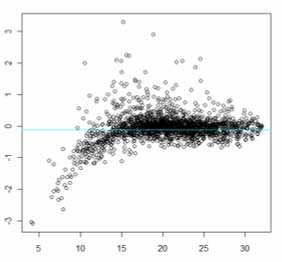
\includegraphics{data/albi_ueb11_a43_mva}
\caption{MvA-Plot}
\label{fig:43}
\end{figure}

\item Die Regression ist in \textcolor{magenta}{violett} eingezeichnet.
Bei der Normalisierung wird der durchschnittliche Abstand zu allen Punkten einer Fensterbreite errechnet.
Je weiter ein Punkt von der entstehenden Regressionslinie entfernt ist, desto stärker wird er durch die Normalisierung verschoben.

\item Der Kernel ermöglicht eine Gewichtung der Punkte, die zur Normalisierung herangezogen werden.
Es kann zum Beispiel eine Normalverteilung als Gewichtung gewählt werden, um solche Punkte, die nahe am zu normalisierenden Punkt liegen,
stärker zu gewichten, als solche, die eine große Distanz zu ihm haben.
\end{enumerate}

\aufgabe{RNA-Struktur}{30}
\begin{enumerate}
\item
Es treten folgende Sekundärstrukturelemente auf:
\begin{itemize}
\item Stacks / helices in allen
\item Bulges in B
\item Hairpin loops in allen
\item Interior loops in B
\item Multi loops in A, C und D
\end{itemize}

\item
Die Struktur C kann so nicht vom Zucker-Algorithmus bestimmt werden,
da sie der Bedingung der Zugänglichkeit widerspricht.
Das zeigt sich deutlich an den sich kreuzenden Linien Abbildung \ref{fig:44b}.

\begin{figure}
\setlength{\unitlength}{1cm}
\centering

\begin{picture}(5,5)(0,0)
\qbezier(0,2.5)(0.2,4.8)(2.5,5)
\qbezier(2.5,5)(4.8,4.8)(5,2.5)
\qbezier(5,2.5)(4.8,0.2)(2.5,0)
\qbezier(2.5,0)(0.2,0.2)(0,2.5)
\end{picture}

\caption{Kreisdiagramm}
\label{fig:44b}
\end{figure}

\end{enumerate}

\aufgabe{Clustering}{40}
\begin{enumerate}
\item
In Tabelle \ref{tab:45a} sind in jeder Spalte die Einträge der Distanzmatrix für die Distanzen möglicher Cluster zueinander eingetragen.
Es wird jeweils das Cluster mit dem kleinsten Wert ausgewählt und die nächste Spalte mittels complete-linkage berechnet.

\begin{table}
\begin{tabular}{|c|cccccc|}
\hline
 	& D & D & D & D & D & D \\\hline\hline
\texttt{AB}	& 3		& 3		& 3		& \texttt{(AB)}	& 		& \\
\texttt{AC}	& 6		& 7		& 7		& 7		& 11	& \texttt{(((AB)((CD)(EF)))}\\
\texttt{AD}	& 7		& s. \texttt{AC}	& 		& 		& 		& \\
\texttt{AE}	& 11	& 11	& 11	& 11	& s. \texttt{AC}	& \\
\texttt{AF}	& 11	& 11	& s. \texttt{AE}	& 		& 		& \\
\texttt{BC}	& 3		& 4		& 4		& s. \texttt{AC}	& 		& \\
\texttt{BD}	& 4		& s. \texttt{BC}	& 		& 		& 		& \\
\texttt{BE}	& 8		& 8		& 8		& s. \texttt{AE}	& 		& \\
\texttt{BF}	& 8		& 8		& s. \texttt{BE}	& 		& 		& \\
\texttt{CD}	& 1		& \texttt{(CD)}	& 		& 		& 		& \\
\texttt{CE}	& 5		& 5		& 5		& 5		& \texttt{((CD)(EF))}	& \\
\texttt{CF}	& 5		& 5		& s. \texttt{CF}	& 		& 		& \\
\texttt{DE}	& 4		& s. \texttt{CE}	& 		& 		& 		& \\
\texttt{DF}	& 4		& s. \texttt{CF}	& 		& 		& 		& \\
\texttt{EF}	& 2		& 2		& \texttt{(EF)}	& 		& 		& \\
\hline
\end{tabular}

\caption{Clustering mit complete-linkage}
\label{tab:45a}
\end{table}

Es ergibt sich daraus schließlich das Clustering \texttt{((AB)((CD)(EF)))}.

\item
Tabelle \ref{tab:45b} ist aufgebaut wie Tabelle \ref{tab:45a}, jedoch werden neue Spalten mit single-linkage berechnet.

\begin{table}
\begin{tabular}{|c|cccccc|}
\hline
 	& D & D & D & D & D & D\\\hline\hline
\texttt{AB}	& 3		& 3		& 3		& \texttt{(AB)}	& 		& \\
\texttt{AC}	& 6		& 6		& 6		& 3		& \texttt{((AB)(CD))}	& \\
\texttt{AD}	& 7		& s. \texttt{AC}	& 		& 		& 		& \\
\texttt{AE}	& 11	& 11	& 11	& 8		& 4		& \texttt{(((AB)(CD))(EF))}\\
\texttt{AF}	& 11	& 11	& s. \texttt{AE}	& 		& 		& \\
\texttt{BC}	& 3		& 3		& 3		& s. \texttt{AC}	& 		& \\
\texttt{BD}	& 4		& s. \texttt{BC}	& 		& 		& 		& \\
\texttt{BE}	& 8		& 8		& 8		& s. \texttt{AE}	& 		& \\
\texttt{BF}	& 8		& 8		& s. \texttt{BE}	& 		& 		& \\
\texttt{CD}	& 1		& \texttt{(CD)}	& 		& 		& 		& \\
\texttt{CE}	& 5		& 4		& 4		& 4		& s. \texttt{AE}	& \\
\texttt{CF}	& 5		& 4		& s. \texttt{CE}	& 		& 		& \\
\texttt{DE}	& 4		& s. \texttt{CE}	& 		& 		& 		& \\
\texttt{DF}	& 4		& s. \texttt{CF}	& 		& 		& 		& \\
\texttt{EF}	& 2		& 2		& \texttt{(EF)}	& 		& 		& \\
\hline
\end{tabular}

\caption{Clustering mit single-linkage}
\label{tab:45b}
\end{table}

Es ergibt sich daraus schließlich das Clustering \texttt{(((AB)(CD))(EF))}.

\item Der Punkt $x$ hat einen nächsten Nachbarn mit Abstand $2$ in $A$ und zwei nächste Nachbarn mit Abständen $2$ und $3$ in $B$.
Der nächstgelegene Punkt aus $A$ hätte dann einen Abstand von $4$. Daher gilt $x \in B$.
\end{enumerate}

\end{enumerate}
\end{document}
